\chapter{Teoria}
\label{ch:teoria}
Tässä osiossa lukijaa perehdytetään työn kannalta tärkeään teoriaan. Teoriaosuuden kokonaan lukemalla lukija ymmärtää mitä IEC 61850 -standardi tarkoittaa sähköasemien kannalta ja mitä kaikkea se määrittää. Kuinka standardi määrittää viestien tilauksen, ja mitä malleja ja palveluita niihin liittyy. Työn lopullisessa toteutuksessa viestit prosessoitiin ja julkaistiin jonopalvelimelle myöhempää käyttöä varten. Teorian lopussa lukija perehdytetään jonopalvelimen toteukseen liityvään teoriaan. Teoriaosuus lukemalla lukija varmistaa että, ymmärtää ohjelmiston suunnittelu- ja toteutusvaiheessa käsitellyt käsitteet ja aiheet.


\section{IEC 61850 -standardi yhteiseen kommunikointiin}
Sähköasemilla nykypäivänä käytössä olevilla älykkäillä elektronisilla laitteilla (engl. Intelligent Electronic Device, lyhennetään IED) toteutetaan aseman toiminnalisuuden funktioita. Aseman toiminnallisuuteen liittyy sen kontrollointi ja suojaus. Aseman komponenttien suojauksen lisäksi, siihen kuuluu myös asemalta lähtevät sähkölinjat. Hyvä esimerkki sähköaseman suojauksesta on korkeajännitelinjan katkaisija, joka katkaisee virran linjasta vikatilanteissa, kuten linjan poikkimeno kaatuneen puun tai pylvään takia. Fyysistä katkaisijaa ohjaa aseman automatiikka, joka toteutetaan IED-laitteilla. Eli IED-laite voi olla kytketty fyysisesti ohjattavaan laitteeseen \cite[s.~63--64]{IEC61850-7-1}. Koko sähköaseman toiminnallisuus koostuu monesta funktiosta, jotka on jaettu monelle IED-laitteelle. Jotta systeemi pystyy toimimaan, täytyy IED-laitteiden kommunikoida keskenään ja vaihtaa informaatiota toistensa kanssa. IED-laitteiden täytyy myös kommunikoida asemalta ulospäin erilliselle ohjausasemalle monitorointia ja etäohjausta varten \cite[s.~1]{Brunner2008}. On selvää, että monimutkaisen systeemin ja monen valmistajien kesken tarvitaan yhteiset säännöt yhteistä kommunikointia varten.

Maailmanlaajuisesti määritetty IEC 61850 -standardi määrittää sähköaseman sisäisen kommunikoinnin IED-laitteiden välillä. Standardi määrittää myös kommunikointisäännöt asemalta lähtevään liikenteeseen, kuten toiselle sähköasemalle ja ohjausasemalle \cite[s.~10]{IEC61850-7-1}. Ilman yhteisiä sääntöjä jokainen valmistaja olisi vapaa toteuttamaan omat säännöt ja protokollat kommunikointiin. Seurauksena tästä olisi, että laitteet eivät olisi keskenään yhteensopivia eri valmistajien välillä. Standardin on tarkoitus poistaa tämä ja määrittää yhteiset pelisäännöt kommunikoinnin toteuttamiseen \cite[s.~1]{Kaneda2008}.

Todella tärkeä ja iso osa standardia on sähköaseman systeemin funktioiden abstrahointi mallien kautta. Standardi määrittää tarkasti kuinka abstraktit mallit määritellään aseman oikeista laiteista ja niiden ominaisuuksista. Tarkoituksena on tehdä mallit tekniikasta ja toteutuksesta riippumattomaksi. Tämän jälkeen abstrahoidut mallit mallinnetaan erikseen jollekin tekniikalle, joka sen mahdollistaa. Abtrahoituja malleja käytetään myös määrittämään sähköaseman IED-laitteiden ja aseman muiden osien konfigurointi. Abstrahoitujen mallien ansiosta standardi on pohjana tulevaisuuden laajennoksille ja tekniikoille. Uusien tekniikoiden ilmaantuessa, voidaan standardin lisätä  osa, joka  mallintaa abstraktimallit kyseiselle tekniikalle \cite[s.~2]{Brunner2008}.


\subsection{Standardin historia}
\begin{it}
	Kirjoita tähän standardin historiaa ja kuinka se muodostui. Pohdi kuitenkin ensin onko tämä lukijan kannalta tärkeää ja tarvittavaa tietoa.
\end{it}


\subsection{Standardin eri osat ja niiden merkitykset}	
IEC 61850 -standardi on todella laaja kokonaisuus. Tämän takia se on pilkottu erillisiin dokumentteihin, josta jokainen käsittelee omaa asiaa. Historian saatossa standardiin on lisätty uusia dokumentteja laajentamaan standardia \cite{IEC61850series, New-documents-by-IEC-TC-57} \cite[s.~13]{IEC61850-1}. Tämän työn kirjoitushetkellä standardiin kuului lisäki paljon muitakin dokumentteja, esimerkiksi uusiin mallinnuksiin muille tekniikoille ja vesivoimalaitoksien mallintamiseen liittyviä dokumentteja. Laajuudesta huolimatta standardin voi esittää 10:llä eri pääkohdalla ja näiden alakohdilla. Taulukossa \ref{tab:iec61850-dokumentin-osat} on esitetty standardin pääkohdan dokumentit ja niiden alkuperäiset englanninkieliset otsikot \cite[s.~2]{Mackiewicz2006} \cite{IEC61850series}. Kuvassa \ref{fig:iec61850-osat-ja-relaatiot} on esitetty kaikki standardin eri osat ja niiden väliset relaatiot toisiinsa. Kuvaan on merkitty yhteinäisellä viivalla ne osat, jotka ovat tämän työn kannalta tärkeitä. Ja katkoviivalla ne, jotka eivät ole.

\begin{table}[ht!]
	\caption{IEC 61850 -standardin pääkohtien ja niiden alakohtien dokumentit.}
	\label{tab:iec61850-dokumentin-osat}
	\begin{tabular}{l | l}
		\hline
		\textbf{Osa} & \textbf{Otsikko englanniksi} \\
		\hline \hline
		1 & Introduction and overview \\
		2 & Glossary \\
		3 & General requirements \\
		4 & System and project management \\
		5 & \parbox[t]{13cm}{Communication requirements for functions and device models} \\
		6 & \parbox[t]{13cm}{Configuration description language for communication in power utility \par automation systems related to IEDs} \\
		7-1 & \parbox[t]{13cm}{Basic communication structure - Principles and models} \\
		7-2 & \parbox[t]{13cm}{Basic information and communication structure - Abstract communication service interface (ACSI)} \\
		7-3 & \parbox[t]{13cm}{Basic communication structure - Common data classes} \\
		7-4 & \parbox[t]{13cm}{Basic communication structure - Compatible logical node classes and data object classes} \\
		8-1 & \parbox[t]{13cm}{Specific communication service mapping (SCSM) - \par  Mappings to MMS (ISO 9506-1 and ISO 9506-2) and to ISO/IEC 8802-3} \\
		9-2 & \parbox[t]{13cm}{Specific communication service mapping (SCSM) - \par  Sampled values over ISO/IEC 8802-3} \\
		9-3 & \parbox[t]{13cm}{Precision time protocol profile for power utility automation} \\
		10 & Conformance testing \\
		\hline
	\end{tabular}
\end{table}

\begin{figure}
	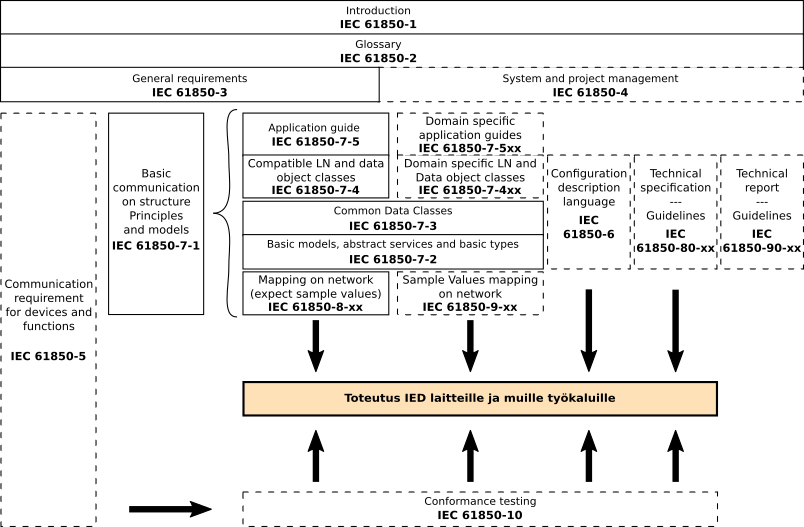
\includegraphics[width=1\textwidth]{pictures/iec61850-series-parts-and-relations.png}
	\caption{IEC 61850 -standardin osat ja niiden väliset relaatiot \cite[s.~14]{IEC61850-7-1} \cite[s.~22]{IEC61850-1}.}
	\label{fig:iec61850-osat-ja-relaatiot}
\end{figure}

Standardin ensimmäiset osat 1--5 kattavat yleistä kuvaa standardista ja sen vaatimuksista. Osiossa 6 käsitellään IED-laitteiden konfigurointiin käytetty XML (engl. Extensible Markup Language) -pohjainen kieli \cite[s.~7--8]{IEC61850-6}. Tämä osuus ei ole tämän työn kannalta tärkeä ja sitä ei sen tarkemmin käsitellä. Osat 7.1--7.4 käsittelevät standardin abstraktia mallia, niiden palveluita ja kuinka se rakentuu. Abstrahoidut palvelut standardissa lyhennetään ACSI (engl. Abstract Communication Service Interface), ja samaa lyhennettä käytetään tässä työssä \cite[s.~72]{IEC61850-7-1}. Osissa 8--9 ja niiden alakohdissa käsitellään abstraktimallien mallintamista erillisille protokollille, jolloin malleista tulee kyseisestä tekniikasta riippuvaisia. Abstrakteja malleja ja niiden mallintamista tekniikalle käsitellään teoriassa erikseen. Osa 10 käsittelee testausmenetelmiä, joilla voidaan varmistaa standardin määritysten noudattaminen. Tämä osuus ei myöskään ole tämän työn kannalta tärkeä, ja sitä ei teoriassa sen takia käsitellä. \cite[s.~15]{IEC61850-7-1}


\subsection{Abstraktimalli ja sen osat}
\begin{it}
	Kirjoita tähän aseman funktioiden, fyysisen laitteiden ja loogisten noodien suhteesta toisiinsa. Kuva myös piirrä ja mallia ja tietoa tähän ota \cite[s.~19]{IEC61850-1}. Tälle tarve jos teksti ei ole muuten tarpeeksi ymmärrettävä.

	Piirrä tähän itse esimerkkikuva kuinka standardi mallintaa fyysisen laitteen loogisiksi laitteiksi. Ota mallia standarin 7-1 kuvasta sivulla 17.
\end{it}

IEC 61850 -standardin lähtökohtana on pilkkoa koko sähköaseman toiminnalisuuden funktiot pieniksi yksilöiksi. Pilkotut yksilöt abstrahoidaan ja pidetään sopivan kokoisina, jotta ne voidaan konfiguroida esitettäväksi erillisellä IED-laiteella. Yksi aseman funktio voidaan hajauttaa monelle eri IED-laitteelle. Esimerkiksi linjan suojaukseen liittyvät komponentit, katkaisija (engl. circuit braker) ja ylivirtasuoja (engl. overcurrent protection) omilla IED-laitteillaan. Toimiakseen, laitteiden täytyy vaihtaa informaatiota keskenään \cite[s.~31]{IEC61850-7-1}. Näitä pilkottuja yksilöitä kutsutaan standardissa nimellä looginen noodi (engl. logical node ja lyhennetään LN). Loogiset noodit siis mallinetaan jostakin systeemin käsiteellisestä osasta. Loogisia noodeja käytetään rakentamaan looginen laite (engl. logic device, lyhennetään LD). Looginen laite on aseman ohjausyksikkö ja jokin fyysisen laitteen osa, joka toteuttaa loogisten noodien ohjauksen yhtäaikaa. Ylläolevasta esimerkistä looginen laite olisi aseman linjan suojaukseen liittyvät osat sisältä laite. Looginen laite siis vastaa aseman fyysistä laitetta, joka on kytketty aseman verkkoon ja sillä on IP-osoite. Yksi aseman fyysinen laite voi hoitaa monen loogisen laitteen funktionaalisuuden. Kuvassa \ref{fig:iec61850-data-modeling} on esitetty standardin mallin eri osien hierarkia ja kuinka ne rakentuvat \cite[s.~2]{Camachi2017} \cite[s.~24]{IEC61850-1}.

\begin{figure}
	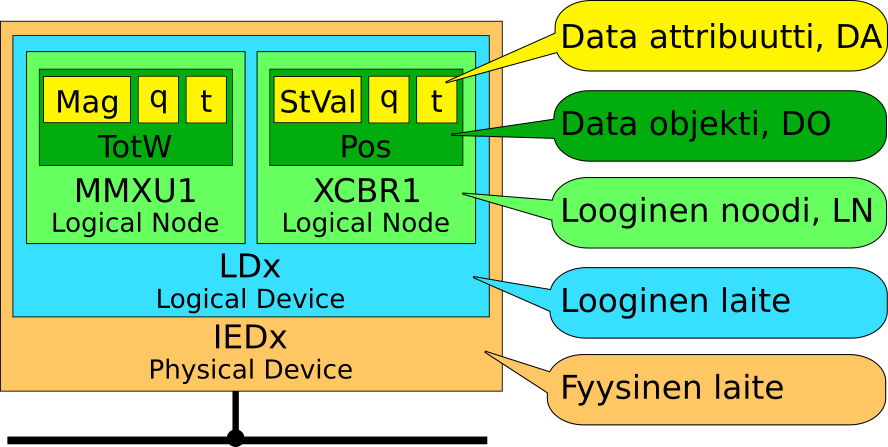
\includegraphics[width=1\textwidth]{pictures/iec61850-data-modeling.png}
	\caption{IEC 61850 -standardin abstraktimallin osat ja niiden hierarkia.}
	\label{fig:iec61850-data-modeling}
\end{figure}

Standardin määrittämissä osien hierarkiassa looginen laite on ylin yksilö, joka sisältää loogisia noodeja. Kuvassa \ref{fig:iec61850-data-modeling} IEDx ja LDx vastaavasti. Looginen noodi sisältää data objekteja (engl. data object, lyhennetään DO). Kuvassa \ref{fig:iec61850-data-modeling} loogiset noodit XCBR1 ja MMXU1. Ja data objektit Pos ja TotW. Data objekti sisältää data attribuutteja (engl. data attribute, lyhennetään DA). Kuvassa \ref{fig:iec61850-data-modeling} StVal, Mag, q ja t. Data objekti on tapa koostaa yhteen samaan asiaan liittyvät data attribuutit. Data attribuutit ovat laitteen konfiguroitavia ja luettavia datapisteitä. Data attribuutit kuvaavat esimerkiksi fyysisen laitteen tilaa ja mittausarvoja. Esimerkiksi mitattua jännitettä tai katkaisimen tilaa (kiinni tai auki). Standardin määrittämät data- objektit ja attribuutit voidaan lajitella 5 eri ryhmään:
\begin{itemize}
	\item yleinen loogisen noodin informaatio,
	\item tila informaatio,
	\item asetukset, 
	\item mitatut arvot ja
	\item ohjaus \cite[s.~25]{IEC61850-1}.
\end{itemize}

Tässä vaiheessa on hyvä mainita, että standardi pyrkii esittämään aseman funktioiden toiminnallisuutta hierarkialla ja oliopohjaisesti. Oliopohjaisesti siten, että standardi määrittää valmiita luokkia erilaisille loogisille noodeille. Esimerkiksi katkaisijalle on määritelty luokka nimeltä XCBR (circuit braker) \cite[s.~105--106]{IEC61850-7-4}. Ja mittaukselle MMXU (measurement) \cite[s.~57--58]{IEC61850-7-4}. Kun aseman toiminnallisuutta esitetään konfiguraatiossa ja IED-laitteella, luokia instanssioidaan tarpeen mukaan. Esimerkiksi kuvassa \ref{fig:iec61850-data-modeling} aikaisemmin mainitut loogisen noodin luokat on instansioitu nimellä XCBR1 ja MMXU1.

Standardi määrittää todella paljon erilaisia valmiita luokkia erilaisille loogisille noodeille valmiina käytettäväksi. Standardi myös määrittää laajenoksien mahdollisuudet luokkia käyttäen. Kaikki määritetyt luokat loogisille noodeille voi löytää standardin osasta 7-4. Kuinka standardi tarkemmin rakentaa luokat ja niiden attribuutit, käsitellään teoriassa omana kohtanaan tuonnempana.


\subsection{Loogisen noodin luokan ja kenttien rakentuminen}
\begin{it}
	Kirjoita tähän kuinka standardin loogiset noodit rakentuvat. Kerro mitä common data classes sisältää ja kuinka ne määrittää data monessa paikassa käytetyt data attribuutit. Tämän jälkeen kuinka loogisen noodin luokat rakennetaan käyttämällä CDC määrityksiä \cite[s.~26]{IEC61850-1}. Ota tähän myös kuvia taulukosta ja rakenna esimerkkinä yksi looginen noodi niitä käyttäen. Tätä samaa mallia voi myöhemmin käyttää määrittämään kuinka referensssipolut luokkien nimillä rakentuu. Tietoa luokkien polkuun voi ottaa täältä ja kuvakin on hyvä \cite[s.~93--95]{IEC61850-7-1}.
	Mallia loogisen noodin rakentamiseen voi myös ottaa \cite[s.~27]{IEC61850-7-1}.

	Kirjoita tähän siitä miten 7-4 osassa on esitetty luokkia ja kuinka ne liittyy 7-3 osan luokkiin. Kuinka näistä muodostetaan instansseja ja mistä arvot tulevat. Tämän jälkeen voisi selittää kuinka polku dataan muodostuu.
\end{it}


\subsection{Abstrakti kommunikointi ja ACSI}
\begin{it}
	Voisiko tähän kirjoittaa miten mappaus johonkin tekniikkaan tapahtuu ja kuinka kommunikaatio sitten tapahtuu oikeasti. Samalla selittää ACSI-mallista jotain. Hyvä kuva standardissa löytyy tästä löytyy \cite[s.~76]{IEC61850-7-1}. Voisiko tämän heittää johonkin omana otsikkonaan?
\end{it}


\subsection{Viestiblokin konfigurointi ja tilaus}
\begin{it}
	Kirjoita tähän IEC 61850 -standardin määrittästä abstraktista raportointimallista. Tätä raportointi mekanismia tullaan käyttämään raporttien tilauksessa ja sen konfigurointi täytyy ymmärtää toteuttettavan ohjelmiston kannalta. Käy läpi mitä asiakasohjelman täytyy tehdä ja mikä on tapahtumien järjestys jotta raportteja voidaan edes tilata.
	Hyvä kuva ja selitys missä järjestyksessä asiat tapahtuu asiakkaan ja serverin välillä. Ja yleistä tietoa raportoinnista löytyy \cite[s.~40--44]{IEC61850-7-1}.
\end{it}


\subsection{Viestin rakenne}
\begin{it}
	Kirjoita tähän standardin määritämästä viestin rakenteesta ja mitä tietoa se sisältää. Kerro myös sen vaihtoehtoisista kentistä.
	Mainitse että standardissa käytetään UTC-aikaa aikakentissä \cite[s.~50]{IEC61850-7-1}.
\end{it}


\section{Abstraktimallin sovitus MMS-protokollaan}
\begin{it}
	Kirjoita kuinka ylempi ACSI sovitetaan MMS-protokollan palveluiksi ja tietotyypeiksi standardin IEC 61850-8-1 osuuden mukaan. Tähän myös miten raportointi toimii MMS-protokollan päällä.
\end{it}


\subsection{MMS-protokolla}
\begin{it}
	Selitä lyhyesti mikä on MMS-protokolla ja vähän sen tietotyypeistä. Tämän tarkoitus on pohjustaa tulevaa IEC 61850 abstraktien olioiden (ACSI) sovitusta tämän protokollan päälle.
\end{it}


\section{Advanced Message Queuing Protocol}
\begin{it}
	Kirjoita tähän AMQP määrittävästä standardista, mikä sen tarkoitus on ja mihin sitä voidaan käyttää.
\end{it}


\subsection{Viestien välitysmekanismit}
\begin{it}
	Mitä mekanismeja AMQP tarjoaa viestien välittämiseen osapuolille. Näitä on jono, reititys suoraan osapuolien välillä ja viestin julkaisu ja tilaaminen.
\end{it}


\subsection{Tilaus ja julkaisu -mallin osat}
\begin{it}
	Kirjoita tähän AMQP tarjoamista viestien julkaisu ja tilaus -mallin osista osapuolten kesken. Kerro mitä eri osat tekevät ja mikä niiden tehtävä viestien välittämisessä on. Englanniksi osia ovat esim. exchange, queue, publisher ja consumer.
\end{it}